\documentclass[twoside]{book}

% Packages required by doxygen
\usepackage{fixltx2e}
\usepackage{calc}
\usepackage{doxygen}
\usepackage[export]{adjustbox} % also loads graphicx
\usepackage{graphicx}
\usepackage[utf8]{inputenc}
\usepackage{makeidx}
\usepackage{multicol}
\usepackage{multirow}
\PassOptionsToPackage{warn}{textcomp}
\usepackage{textcomp}
\usepackage[nointegrals]{wasysym}
\usepackage[table]{xcolor}

% Font selection
\usepackage[T1]{fontenc}
\usepackage[scaled=.90]{helvet}
\usepackage{courier}
\usepackage{amssymb}
\usepackage{sectsty}
\renewcommand{\familydefault}{\sfdefault}
\allsectionsfont{%
  \fontseries{bc}\selectfont%
  \color{darkgray}%
}
\renewcommand{\DoxyLabelFont}{%
  \fontseries{bc}\selectfont%
  \color{darkgray}%
}
\newcommand{\+}{\discretionary{\mbox{\scriptsize$\hookleftarrow$}}{}{}}

% Page & text layout
\usepackage{geometry}
\geometry{%
  a4paper,%
  top=2.5cm,%
  bottom=2.5cm,%
  left=2.5cm,%
  right=2.5cm%
}
\tolerance=750
\hfuzz=15pt
\hbadness=750
\setlength{\emergencystretch}{15pt}
\setlength{\parindent}{0cm}
\setlength{\parskip}{3ex plus 2ex minus 2ex}
\makeatletter
\renewcommand{\paragraph}{%
  \@startsection{paragraph}{4}{0ex}{-1.0ex}{1.0ex}{%
    \normalfont\normalsize\bfseries\SS@parafont%
  }%
}
\renewcommand{\subparagraph}{%
  \@startsection{subparagraph}{5}{0ex}{-1.0ex}{1.0ex}{%
    \normalfont\normalsize\bfseries\SS@subparafont%
  }%
}
\makeatother

% Headers & footers
\usepackage{fancyhdr}
\pagestyle{fancyplain}
\fancyhead[LE]{\fancyplain{}{\bfseries\thepage}}
\fancyhead[CE]{\fancyplain{}{}}
\fancyhead[RE]{\fancyplain{}{\bfseries\leftmark}}
\fancyhead[LO]{\fancyplain{}{\bfseries\rightmark}}
\fancyhead[CO]{\fancyplain{}{}}
\fancyhead[RO]{\fancyplain{}{\bfseries\thepage}}
\fancyfoot[LE]{\fancyplain{}{}}
\fancyfoot[CE]{\fancyplain{}{}}
\fancyfoot[RE]{\fancyplain{}{\bfseries\scriptsize Generated by Doxygen }}
\fancyfoot[LO]{\fancyplain{}{\bfseries\scriptsize Generated by Doxygen }}
\fancyfoot[CO]{\fancyplain{}{}}
\fancyfoot[RO]{\fancyplain{}{}}
\renewcommand{\footrulewidth}{0.4pt}
\renewcommand{\chaptermark}[1]{%
  \markboth{#1}{}%
}
\renewcommand{\sectionmark}[1]{%
  \markright{\thesection\ #1}%
}

% Indices & bibliography
\usepackage{natbib}
\usepackage[titles]{tocloft}
\setcounter{tocdepth}{3}
\setcounter{secnumdepth}{5}
\makeindex

% Hyperlinks (required, but should be loaded last)
\usepackage{ifpdf}
\ifpdf
  \usepackage[pdftex,pagebackref=true]{hyperref}
\else
  \usepackage[ps2pdf,pagebackref=true]{hyperref}
\fi
\hypersetup{%
  colorlinks=true,%
  linkcolor=blue,%
  citecolor=blue,%
  unicode%
}

% Custom commands
\newcommand{\clearemptydoublepage}{%
  \newpage{\pagestyle{empty}\cleardoublepage}%
}

\usepackage{caption}
\captionsetup{labelsep=space,justification=centering,font={bf},singlelinecheck=off,skip=4pt,position=top}

%===== C O N T E N T S =====

\begin{document}

% Titlepage & ToC
\hypersetup{pageanchor=false,
             bookmarksnumbered=true,
             pdfencoding=unicode
            }
\pagenumbering{roman}
\begin{titlepage}
\vspace*{7cm}
\begin{center}%
{\Large Efficio Runtime C++ \\[1ex]\large 0.\+0.\+0.\+1 }\\
\vspace*{1cm}
{\large Generated by Doxygen 1.8.11}\\
\end{center}
\end{titlepage}
\clearemptydoublepage
\tableofcontents
\clearemptydoublepage
\pagenumbering{arabic}
\hypersetup{pageanchor=true}

%--- Begin generated contents ---
\chapter{Efficio Runtime for C++}
\label{index}\hypertarget{index}{}\section*{Efficio\+C\+PP}

Experimentation with Efficio in C++

\subsection*{For Developers }

The Efficio Runtime project automatically documents itself in a post-\/build step using \href{http://doxygen.org/}{\tt Doxygen}. To take advantage of the documenting feature, simply add the doxygen executables to the Windows P\+A\+TH environment variable. The current documentation can be found \href{https://htmlpreview.github.io/?https://raw.githubusercontent.com/Abantech/EfficioCPP/master/EfficioRuntime/doc/html/index.html}{\tt here} 
\chapter{R\+E\+A\+D\+ME}
\label{md_README}
\hypertarget{md_README}{}
\#\+Efficio C++ The Efficio C++ project is the base on which all other language projects are built.

\section*{Getting the Project to Build in Visual Studio }


\begin{DoxyEnumerate}
\item Download \href{http://swig.org/download}{\tt S\+W\+IG} for Windows v3.\+0.\+10.
\end{DoxyEnumerate}
\begin{DoxyEnumerate}
\item Add S\+W\+IG to the Path environment variable.
\end{DoxyEnumerate}
\begin{DoxyEnumerate}
\item Download \href{http://doxygen.org}{\tt Doxygen}.
\end{DoxyEnumerate}
\begin{DoxyEnumerate}
\item Add Doxygen to the Path environment variable.
\end{DoxyEnumerate}
\begin{DoxyEnumerate}
\item Download the Leap Motion S\+DK.
\end{DoxyEnumerate}
\begin{DoxyEnumerate}
\item Create an environment variable called L\+E\+A\+P\+\_\+\+S\+DK pointing to the Leap Motion S\+DK.
\end{DoxyEnumerate}
\begin{DoxyEnumerate}
\item When the project is compiled .cxx files will be generated or overwritten for each given target language. Make sure these are writable and if generated for the first time, are included in the vcxproj 
\end{DoxyEnumerate}
\chapter{Hierarchical Index}
\section{Class Hierarchy}
This inheritance list is sorted roughly, but not completely, alphabetically\+:\begin{DoxyCompactList}
\item \contentsline{section}{Efficio\+:\+:Body}{\pageref{class_efficio_1_1_body}}{}
\item \contentsline{section}{Efficio\+:\+:Configuration\+:\+:Device\+Configuration}{\pageref{class_efficio_1_1_configuration_1_1_device_configuration}}{}
\item \contentsline{section}{Efficio\+:\+:Engine}{\pageref{class_efficio_1_1_engine}}{}
\item \contentsline{section}{Efficio\+:\+:Events\+:\+:Event}{\pageref{class_efficio_1_1_events_1_1_event}}{}
\begin{DoxyCompactList}
\item \contentsline{section}{Efficio\+:\+:Input\+Recognition\+:\+:Gesture}{\pageref{class_efficio_1_1_input_recognition_1_1_gesture}}{}
\begin{DoxyCompactList}
\item \contentsline{section}{Efficio\+:\+:Input\+Recognition\+:\+:Continuous\+Gesture}{\pageref{class_efficio_1_1_input_recognition_1_1_continuous_gesture}}{}
\item \contentsline{section}{Efficio\+:\+:Input\+Recognition\+:\+:Discrete\+Gesture}{\pageref{class_efficio_1_1_input_recognition_1_1_discrete_gesture}}{}
\begin{DoxyCompactList}
\item \contentsline{section}{Efficio\+:\+:Input\+Recognition\+:\+:Human\+:\+:Hands\+:\+:Pinch}{\pageref{class_efficio_1_1_input_recognition_1_1_human_1_1_hands_1_1_pinch}}{}
\end{DoxyCompactList}
\end{DoxyCompactList}
\end{DoxyCompactList}
\item \contentsline{section}{Efficio\+:\+:Body\+:\+:Finger}{\pageref{class_efficio_1_1_body_1_1_finger}}{}
\item \contentsline{section}{Efficio\+:\+:Finger\+Joint}{\pageref{class_efficio_1_1_finger_joint}}{}
\item \contentsline{section}{Efficio\+:\+:Frame}{\pageref{class_efficio_1_1_frame}}{}
\begin{DoxyCompactList}
\item \contentsline{section}{Efficio\+:\+:Efficio\+Frame}{\pageref{class_efficio_1_1_efficio_frame}}{}
\end{DoxyCompactList}
\item \contentsline{section}{Efficio\+:\+:Body\+:\+:Hand}{\pageref{class_efficio_1_1_body_1_1_hand}}{}
\item \contentsline{section}{Efficio\+:\+:Hand\+Joint}{\pageref{class_efficio_1_1_hand_joint}}{}
\begin{DoxyCompactList}
\item \contentsline{section}{Efficio\+:\+:C\+MC}{\pageref{class_efficio_1_1_c_m_c}}{}
\item \contentsline{section}{Efficio\+:\+:D\+IP}{\pageref{class_efficio_1_1_d_i_p}}{}
\item \contentsline{section}{Efficio\+:\+:IP}{\pageref{class_efficio_1_1_i_p}}{}
\item \contentsline{section}{Efficio\+:\+:I\+P\+C\+MC}{\pageref{class_efficio_1_1_i_p_c_m_c}}{}
\item \contentsline{section}{Efficio\+:\+:M\+CP}{\pageref{class_efficio_1_1_m_c_p}}{}
\item \contentsline{section}{Efficio\+:\+:P\+IP}{\pageref{class_efficio_1_1_p_i_p}}{}
\end{DoxyCompactList}
\item \contentsline{section}{Efficio\+:\+:Historical\+Frame\+Collection}{\pageref{class_efficio_1_1_historical_frame_collection}}{}
\item \contentsline{section}{Efficio\+:\+:Configuration\+:\+:Leap\+Configuration}{\pageref{class_efficio_1_1_configuration_1_1_leap_configuration}}{}
\item \contentsline{section}{Efficio\+:\+:Input\+Recognition\+:\+:Human\+:\+:Hands\+:\+:Single\+Hand\+Gesture}{\pageref{class_efficio_1_1_input_recognition_1_1_human_1_1_hands_1_1_single_hand_gesture}}{}
\item \contentsline{section}{Efficio\+:\+:Input\+Recognition\+:\+:Human\+:\+:Hands\+:\+:Single\+Hand\+Gesture\+Detector}{\pageref{class_efficio_1_1_input_recognition_1_1_human_1_1_hands_1_1_single_hand_gesture_detector}}{}
\item \contentsline{section}{Efficio\+:\+:Skeletal\+Data}{\pageref{class_efficio_1_1_skeletal_data}}{}
\item \contentsline{section}{S\+W\+I\+G\+\_\+\+Java\+Exceptions\+\_\+t}{\pageref{struct_s_w_i_g___java_exceptions__t}}{}
\item \contentsline{section}{S\+W\+I\+G\+\_\+null\+\_\+deleter}{\pageref{struct_s_w_i_g__null__deleter}}{}
\item \contentsline{section}{Efficio\+:\+:Vector3}{\pageref{class_efficio_1_1_vector3}}{}
\end{DoxyCompactList}

\chapter{Class Index}
\section{Class List}
Here are the classes, structs, unions and interfaces with brief descriptions\+:\begin{DoxyCompactList}
\item\contentsline{section}{\hyperlink{class_efficio_1_1_models_1_1_human_1_1_bone2}{Efficio\+::\+Models\+::\+Human\+::\+Bone2} }{\pageref{class_efficio_1_1_models_1_1_human_1_1_bone2}}{}
\item\contentsline{section}{\hyperlink{class_efficio_1_1_input_recognition_1_1_continuous_gesture}{Efficio\+::\+Input\+Recognition\+::\+Continuous\+Gesture} \\*Continuous gestures are gestures that are done over time }{\pageref{class_efficio_1_1_input_recognition_1_1_continuous_gesture}}{}
\item\contentsline{section}{\hyperlink{class_efficio_1_1_device}{Efficio\+::\+Device} \\*Any device which can feel data into Efficio }{\pageref{class_efficio_1_1_device}}{}
\item\contentsline{section}{\hyperlink{class_efficio_1_1_configuration_1_1_device_configuration}{Efficio\+::\+Configuration\+::\+Device\+Configuration} \\*The device configuration is used to configure the devices with which Efficio can work }{\pageref{class_efficio_1_1_configuration_1_1_device_configuration}}{}
\item\contentsline{section}{\hyperlink{class_efficio_1_1_device_manager}{Efficio\+::\+Device\+Manager} \\*Manages all the devices connected to Efficio }{\pageref{class_efficio_1_1_device_manager}}{}
\item\contentsline{section}{\hyperlink{class_efficio_1_1_input_recognition_1_1_discrete_gesture}{Efficio\+::\+Input\+Recognition\+::\+Discrete\+Gesture} \\*Discrete gestures are gestures that are always in a completed state }{\pageref{class_efficio_1_1_input_recognition_1_1_discrete_gesture}}{}
\item\contentsline{section}{\hyperlink{class_efficio_1_1_efficio_frame}{Efficio\+::\+Efficio\+Frame} \\*Object containing all processed and raw signals }{\pageref{class_efficio_1_1_efficio_frame}}{}
\item\contentsline{section}{\hyperlink{class_efficio_1_1_engine}{Efficio\+::\+Engine} \\*Efficio engine for retrieving processed frames }{\pageref{class_efficio_1_1_engine}}{}
\item\contentsline{section}{\hyperlink{class_efficio_1_1_events_1_1_event}{Efficio\+::\+Events\+::\+Event} \\*The abstract class for all events within the Efficio system. Events are raised when anything notable happens within the Efficio ecosystem }{\pageref{class_efficio_1_1_events_1_1_event}}{}
\item\contentsline{section}{\hyperlink{class_efficio_1_1_models_1_1_human_1_1_finger}{Efficio\+::\+Models\+::\+Human\+::\+Finger} }{\pageref{class_efficio_1_1_models_1_1_human_1_1_finger}}{}
\item\contentsline{section}{\hyperlink{class_efficio_1_1_models_1_1_human_1_1_finger_joint}{Efficio\+::\+Models\+::\+Human\+::\+Finger\+Joint} }{\pageref{class_efficio_1_1_models_1_1_human_1_1_finger_joint}}{}
\item\contentsline{section}{\hyperlink{class_efficio_1_1_frame}{Efficio\+::\+Frame} }{\pageref{class_efficio_1_1_frame}}{}
\item\contentsline{section}{\hyperlink{class_efficio_1_1_input_recognition_1_1_gesture}{Efficio\+::\+Input\+Recognition\+::\+Gesture} \\*Base class for all gestures that may occur within the Efficio system }{\pageref{class_efficio_1_1_input_recognition_1_1_gesture}}{}
\item\contentsline{section}{\hyperlink{class_efficio_1_1_models_1_1_human_1_1_hand}{Efficio\+::\+Models\+::\+Human\+::\+Hand} }{\pageref{class_efficio_1_1_models_1_1_human_1_1_hand}}{}
\item\contentsline{section}{\hyperlink{class_efficio_1_1_hand_data}{Efficio\+::\+Hand\+Data} }{\pageref{class_efficio_1_1_hand_data}}{}
\item\contentsline{section}{\hyperlink{class_efficio_1_1_historical_frame_collection}{Efficio\+::\+Historical\+Frame\+Collection} \\*Collection of historical Efficio frames }{\pageref{class_efficio_1_1_historical_frame_collection}}{}
\item\contentsline{section}{\hyperlink{class_efficio_1_1_models_1_1_human_1_1_joint}{Efficio\+::\+Models\+::\+Human\+::\+Joint} }{\pageref{class_efficio_1_1_models_1_1_human_1_1_joint}}{}
\item\contentsline{section}{\hyperlink{class_efficio_1_1_configuration_1_1_leap_configuration}{Efficio\+::\+Configuration\+::\+Leap\+Configuration} \\*Configuration for the Leap Motion device }{\pageref{class_efficio_1_1_configuration_1_1_leap_configuration}}{}
\item\contentsline{section}{\hyperlink{class_efficio_1_1_leap_motion_device}{Efficio\+::\+Leap\+Motion\+Device} }{\pageref{class_efficio_1_1_leap_motion_device}}{}
\item\contentsline{section}{\hyperlink{class_efficio_1_1_input_recognition_1_1_human_1_1_hands_1_1_pinch}{Efficio\+::\+Input\+Recognition\+::\+Human\+::\+Hands\+::\+Pinch} }{\pageref{class_efficio_1_1_input_recognition_1_1_human_1_1_hands_1_1_pinch}}{}
\item\contentsline{section}{\hyperlink{class_efficio_1_1_input_recognition_1_1_human_1_1_hands_1_1_pinch_detector}{Efficio\+::\+Input\+Recognition\+::\+Human\+::\+Hands\+::\+Pinch\+Detector} }{\pageref{class_efficio_1_1_input_recognition_1_1_human_1_1_hands_1_1_pinch_detector}}{}
\item\contentsline{section}{\hyperlink{class_efficio_1_1_input_recognition_1_1_human_1_1_hands_1_1_single_hand_gesture}{Efficio\+::\+Input\+Recognition\+::\+Human\+::\+Hands\+::\+Single\+Hand\+Gesture} }{\pageref{class_efficio_1_1_input_recognition_1_1_human_1_1_hands_1_1_single_hand_gesture}}{}
\item\contentsline{section}{\hyperlink{class_efficio_1_1_input_recognition_1_1_human_1_1_hands_1_1_single_hand_gesture_detector}{Efficio\+::\+Input\+Recognition\+::\+Human\+::\+Hands\+::\+Single\+Hand\+Gesture\+Detector} }{\pageref{class_efficio_1_1_input_recognition_1_1_human_1_1_hands_1_1_single_hand_gesture_detector}}{}
\item\contentsline{section}{\hyperlink{struct_s_w_i_g___c_sharp_exception__t}{S\+W\+I\+G\+\_\+\+C\+Sharp\+Exception\+\_\+t} }{\pageref{struct_s_w_i_g___c_sharp_exception__t}}{}
\item\contentsline{section}{\hyperlink{struct_s_w_i_g___c_sharp_exception_argument__t}{S\+W\+I\+G\+\_\+\+C\+Sharp\+Exception\+Argument\+\_\+t} }{\pageref{struct_s_w_i_g___c_sharp_exception_argument__t}}{}
\item\contentsline{section}{\hyperlink{struct_s_w_i_g___java_exceptions__t}{S\+W\+I\+G\+\_\+\+Java\+Exceptions\+\_\+t} }{\pageref{struct_s_w_i_g___java_exceptions__t}}{}
\item\contentsline{section}{\hyperlink{struct_s_w_i_g__null__deleter}{S\+W\+I\+G\+\_\+null\+\_\+deleter} }{\pageref{struct_s_w_i_g__null__deleter}}{}
\item\contentsline{section}{\hyperlink{class_efficio_1_1_vector3}{Efficio\+::\+Vector3} }{\pageref{class_efficio_1_1_vector3}}{}
\end{DoxyCompactList}

\chapter{Class Documentation}
\hypertarget{class_efficio_1_1_configuration_1_1_device_configuration}{}\section{Efficio\+:\+:Configuration\+:\+:Device\+Configuration Class Reference}
\label{class_efficio_1_1_configuration_1_1_device_configuration}\index{Efficio\+::\+Configuration\+::\+Device\+Configuration@{Efficio\+::\+Configuration\+::\+Device\+Configuration}}


The device configuration is used to configure the devices with which Efficio can work.  




{\ttfamily \#include $<$Device\+Configuration.\+h$>$}

\subsection*{Public Attributes}
\begin{DoxyCompactItemize}
\item 
\hyperlink{class_efficio_1_1_configuration_1_1_leap_configuration}{Leap\+Configuration} \hyperlink{class_efficio_1_1_configuration_1_1_device_configuration_aa5c43ffa75c5483880a21ef3490b54d6}{Leap\+Configuration}\hypertarget{class_efficio_1_1_configuration_1_1_device_configuration_aa5c43ffa75c5483880a21ef3490b54d6}{}\label{class_efficio_1_1_configuration_1_1_device_configuration_aa5c43ffa75c5483880a21ef3490b54d6}

\begin{DoxyCompactList}\small\item\em The configuration for the Leap Motion. \end{DoxyCompactList}\end{DoxyCompactItemize}


\subsection{Detailed Description}
The device configuration is used to configure the devices with which Efficio can work. 

The documentation for this class was generated from the following files\+:\begin{DoxyCompactItemize}
\item 
Device\+Configuration.\+h\item 
Device\+Configuration.\+cpp\end{DoxyCompactItemize}

\hypertarget{class_efficio_1_1_efficio_frame}{}\section{Efficio\+:\+:Efficio\+Frame Class Reference}
\label{class_efficio_1_1_efficio_frame}\index{Efficio\+::\+Efficio\+Frame@{Efficio\+::\+Efficio\+Frame}}


Object containing all processed and raw signals.  




{\ttfamily \#include $<$Efficio\+Frame.\+h$>$}

\subsection*{Public Member Functions}
\begin{DoxyCompactItemize}
\item 
{\bfseries Efficio\+Frame} (int ID)\hypertarget{class_efficio_1_1_efficio_frame_a9b49dc8882fa2c58ebcd8710bb14de91}{}\label{class_efficio_1_1_efficio_frame_a9b49dc8882fa2c58ebcd8710bb14de91}

\item 
std\+::vector$<$ std\+::shared\+\_\+ptr$<$ \hyperlink{class_efficio_1_1_events_1_1_event}{Efficio\+::\+Events\+::\+Event} $>$ $>$ {\bfseries Get\+Events} ()\hypertarget{class_efficio_1_1_efficio_frame_a219e88c37091c04515e7022c65300654}{}\label{class_efficio_1_1_efficio_frame_a219e88c37091c04515e7022c65300654}

\item 
std\+::vector$<$ std\+::shared\+\_\+ptr$<$ \hyperlink{class_efficio_1_1_models_1_1_human_1_1_hand}{Efficio\+::\+Models\+::\+Human\+::\+Hand} $>$ $>$ {\bfseries Get\+Hands} ()\hypertarget{class_efficio_1_1_efficio_frame_a2d6b1d6242890666e52a9d09bca6d610}{}\label{class_efficio_1_1_efficio_frame_a2d6b1d6242890666e52a9d09bca6d610}

\item 
void {\bfseries Add\+Event} (std\+::shared\+\_\+ptr$<$ \hyperlink{class_efficio_1_1_events_1_1_event}{Efficio\+::\+Events\+::\+Event} $>$ event\+Ptr)\hypertarget{class_efficio_1_1_efficio_frame_a2a50c673ea34e5d85707a55099ebae63}{}\label{class_efficio_1_1_efficio_frame_a2a50c673ea34e5d85707a55099ebae63}

\item 
void {\bfseries Add\+Hand} (std\+::shared\+\_\+ptr$<$ \hyperlink{class_efficio_1_1_models_1_1_human_1_1_hand}{Efficio\+::\+Models\+::\+Human\+::\+Hand} $>$ hand\+Ptr)\hypertarget{class_efficio_1_1_efficio_frame_aa8aba8a6ee0efc3194b9a9065b932fb2}{}\label{class_efficio_1_1_efficio_frame_aa8aba8a6ee0efc3194b9a9065b932fb2}

\end{DoxyCompactItemize}
\subsection*{Public Attributes}
\begin{DoxyCompactItemize}
\item 
int {\bfseries ID}\hypertarget{class_efficio_1_1_efficio_frame_aa994a72ec58afb3b6b64b9e05a9d0ba9}{}\label{class_efficio_1_1_efficio_frame_aa994a72ec58afb3b6b64b9e05a9d0ba9}

\end{DoxyCompactItemize}


\subsection{Detailed Description}
Object containing all processed and raw signals. 

The documentation for this class was generated from the following files\+:\begin{DoxyCompactItemize}
\item 
Efficio\+Frame.\+h\item 
Efficio\+Frame.\+cpp\end{DoxyCompactItemize}

\hypertarget{class_efficio_1_1_engine}{}\section{Efficio\+:\+:Engine Class Reference}
\label{class_efficio_1_1_engine}\index{Efficio\+::\+Engine@{Efficio\+::\+Engine}}


Efficio engine for retrieving processed frames.  




{\ttfamily \#include $<$Engine.\+h$>$}

\subsection*{Public Member Functions}
\begin{DoxyCompactItemize}
\item 
void {\bfseries Start} ()\hypertarget{class_efficio_1_1_engine_a3b6e5c963c14df6e902f72df6a521fd1}{}\label{class_efficio_1_1_engine_a3b6e5c963c14df6e902f72df6a521fd1}

\item 
std\+::shared\+\_\+ptr$<$ \hyperlink{class_efficio_1_1_efficio_frame}{Efficio\+::\+Efficio\+Frame} $>$ \hyperlink{class_efficio_1_1_engine_a4f46a611516d157a32005a860128f9dc}{Get\+Frame} ()
\item 
std\+::shared\+\_\+ptr$<$ \hyperlink{class_efficio_1_1_efficio_frame}{Efficio\+::\+Efficio\+Frame} $>$ \hyperlink{class_efficio_1_1_engine_a9f81b122b1c2f768110675a79a842117}{Get\+Frame} (int count)
\end{DoxyCompactItemize}
\subsection*{Public Attributes}
\begin{DoxyCompactItemize}
\item 
\hyperlink{class_efficio_1_1_configuration_1_1_device_configuration}{Efficio\+::\+Configuration\+::\+Device\+Configuration} \hyperlink{class_efficio_1_1_engine_afbaba10c9c508bdcc16625a2e51a6148}{Device\+Configuration}\hypertarget{class_efficio_1_1_engine_afbaba10c9c508bdcc16625a2e51a6148}{}\label{class_efficio_1_1_engine_afbaba10c9c508bdcc16625a2e51a6148}

\begin{DoxyCompactList}\small\item\em The device configuration for Efficio. \end{DoxyCompactList}\item 
\hyperlink{class_efficio_1_1_device_manager}{Efficio\+::\+Device\+Manager} \hyperlink{class_efficio_1_1_engine_a09180d13f06e554000ada9f10c62065c}{Device\+Manager}\hypertarget{class_efficio_1_1_engine_a09180d13f06e554000ada9f10c62065c}{}\label{class_efficio_1_1_engine_a09180d13f06e554000ada9f10c62065c}

\begin{DoxyCompactList}\small\item\em The \hyperlink{class_efficio_1_1_device}{Device} Manager. \end{DoxyCompactList}\end{DoxyCompactItemize}


\subsection{Detailed Description}
Efficio engine for retrieving processed frames. 

\subsection{Member Function Documentation}
\index{Efficio\+::\+Engine@{Efficio\+::\+Engine}!Get\+Frame@{Get\+Frame}}
\index{Get\+Frame@{Get\+Frame}!Efficio\+::\+Engine@{Efficio\+::\+Engine}}
\subsubsection[{\texorpdfstring{Get\+Frame()}{GetFrame()}}]{\setlength{\rightskip}{0pt plus 5cm}std\+::shared\+\_\+ptr$<$ {\bf Efficio\+::\+Efficio\+Frame} $>$ Efficio\+::\+Engine\+::\+Get\+Frame (
\begin{DoxyParamCaption}
{}
\end{DoxyParamCaption}
)}\hypertarget{class_efficio_1_1_engine_a4f46a611516d157a32005a860128f9dc}{}\label{class_efficio_1_1_engine_a4f46a611516d157a32005a860128f9dc}
Gets the current \hyperlink{class_efficio_1_1_efficio_frame}{frame} from the runtime. \begin{DoxyReturn}{Returns}
the current frame. 
\end{DoxyReturn}
\index{Efficio\+::\+Engine@{Efficio\+::\+Engine}!Get\+Frame@{Get\+Frame}}
\index{Get\+Frame@{Get\+Frame}!Efficio\+::\+Engine@{Efficio\+::\+Engine}}
\subsubsection[{\texorpdfstring{Get\+Frame(int count)}{GetFrame(int count)}}]{\setlength{\rightskip}{0pt plus 5cm}std\+::shared\+\_\+ptr$<$ {\bf Efficio\+::\+Efficio\+Frame} $>$ Efficio\+::\+Engine\+::\+Get\+Frame (
\begin{DoxyParamCaption}
\item[{int}]{count}
\end{DoxyParamCaption}
)}\hypertarget{class_efficio_1_1_engine_a9f81b122b1c2f768110675a79a842117}{}\label{class_efficio_1_1_engine_a9f81b122b1c2f768110675a79a842117}
Gets the historical \hyperlink{class_efficio_1_1_efficio_frame}{frame} from the runtime. \begin{DoxyReturn}{Returns}
the current frame. 
\end{DoxyReturn}


The documentation for this class was generated from the following files\+:\begin{DoxyCompactItemize}
\item 
Engine.\+h\item 
Engine.\+cpp\end{DoxyCompactItemize}

\hypertarget{class_efficio_1_1_event}{}\section{Efficio\+:\+:Event Class Reference}
\label{class_efficio_1_1_event}\index{Efficio\+::\+Event@{Efficio\+::\+Event}}


The abstract class for all events within the Efficio system. Events are raised when anything notable happens within the Efficio ecosystem.  




{\ttfamily \#include $<$Event.\+h$>$}

Inheritance diagram for Efficio\+:\+:Event\+:\begin{figure}[H]
\begin{center}
\leavevmode
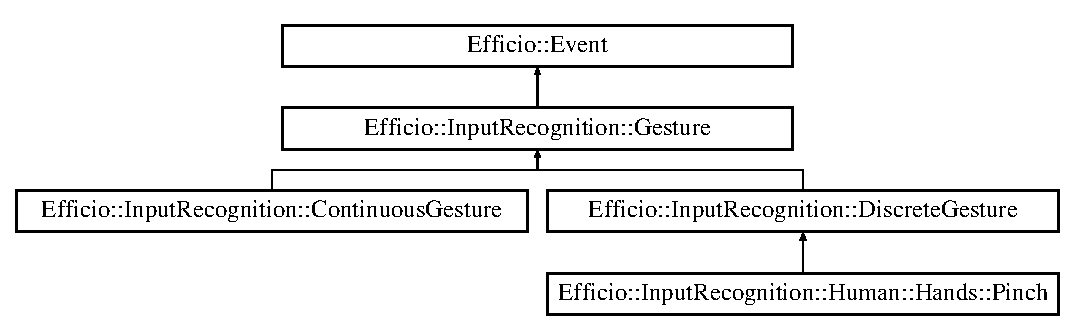
\includegraphics[height=4.000000cm]{class_efficio_1_1_event}
\end{center}
\end{figure}


\subsection{Detailed Description}
The abstract class for all events within the Efficio system. Events are raised when anything notable happens within the Efficio ecosystem. 

The documentation for this class was generated from the following files\+:\begin{DoxyCompactItemize}
\item 
Event.\+h\item 
Event.\+cpp\end{DoxyCompactItemize}

\hypertarget{class_efficio_1_1_frame}{}\section{Efficio\+:\+:Frame Class Reference}
\label{class_efficio_1_1_frame}\index{Efficio\+::\+Frame@{Efficio\+::\+Frame}}
\subsection*{Public Member Functions}
\begin{DoxyCompactItemize}
\item 
\hyperlink{class_efficio_1_1_data_1_1_datum}{Efficio\+::\+Data\+::\+Datum} $\ast$ {\bfseries Get\+Data} (Efficio\+::\+Data\+::\+Datum\+Type data\+Type)\hypertarget{class_efficio_1_1_frame_a8e93ddb6f0dd2b69d56536f673bbc29c}{}\label{class_efficio_1_1_frame_a8e93ddb6f0dd2b69d56536f673bbc29c}

\item 
void {\bfseries Add\+Data} (\hyperlink{class_efficio_1_1_data_1_1_datum}{Efficio\+::\+Data\+::\+Datum} $\ast$datum)\hypertarget{class_efficio_1_1_frame_a75ccb8867d8acfe698073a67f33f72d4}{}\label{class_efficio_1_1_frame_a75ccb8867d8acfe698073a67f33f72d4}

\end{DoxyCompactItemize}
\subsection*{Public Attributes}
\begin{DoxyCompactItemize}
\item 
\hyperlink{class_efficio_1_1_hand_data}{Efficio\+::\+Hand\+Data} {\bfseries Hand\+Data}\hypertarget{class_efficio_1_1_frame_a546f841f8294491f08c83ef16e5b421c}{}\label{class_efficio_1_1_frame_a546f841f8294491f08c83ef16e5b421c}

\end{DoxyCompactItemize}


The documentation for this class was generated from the following files\+:\begin{DoxyCompactItemize}
\item 
Frame.\+h\item 
Frame.\+cpp\end{DoxyCompactItemize}

\hypertarget{class_efficio_1_1_configuration_1_1_leap_configuration}{}\section{Efficio\+:\+:Configuration\+:\+:Leap\+Configuration Class Reference}
\label{class_efficio_1_1_configuration_1_1_leap_configuration}\index{Efficio\+::\+Configuration\+::\+Leap\+Configuration@{Efficio\+::\+Configuration\+::\+Leap\+Configuration}}
\subsection*{Public Attributes}
\begin{DoxyCompactItemize}
\item 
bool {\bfseries Enabled}\hypertarget{class_efficio_1_1_configuration_1_1_leap_configuration_a237eb567a1666e71d13e93bb2e9d86a9}{}\label{class_efficio_1_1_configuration_1_1_leap_configuration_a237eb567a1666e71d13e93bb2e9d86a9}

\end{DoxyCompactItemize}


The documentation for this class was generated from the following files\+:\begin{DoxyCompactItemize}
\item 
Leap\+Configuration.\+h\item 
Leap\+Configuration.\+cpp\end{DoxyCompactItemize}

\hypertarget{class_efficio_1_1_body_1_1_hands_1_1_pinch_event}{}\section{Efficio\+:\+:Body\+:\+:Hands\+:\+:Pinch\+Event Class Reference}
\label{class_efficio_1_1_body_1_1_hands_1_1_pinch_event}\index{Efficio\+::\+Body\+::\+Hands\+::\+Pinch\+Event@{Efficio\+::\+Body\+::\+Hands\+::\+Pinch\+Event}}


The event raised when a pinch is detected from one of the devices tracking hands.  




{\ttfamily \#include $<$Pinch\+Event.\+h$>$}

Inheritance diagram for Efficio\+:\+:Body\+:\+:Hands\+:\+:Pinch\+Event\+:\begin{figure}[H]
\begin{center}
\leavevmode
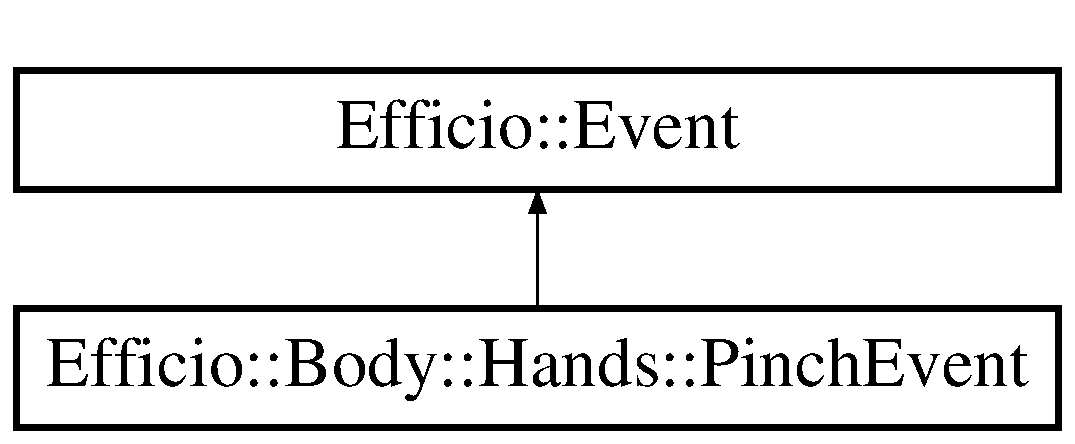
\includegraphics[height=2.000000cm]{class_efficio_1_1_body_1_1_hands_1_1_pinch_event}
\end{center}
\end{figure}
\subsection*{Public Member Functions}
\begin{DoxyCompactItemize}
\item 
{\bfseries Pinch\+Event} (Body\+Side side, \hyperlink{class_efficio_1_1_vector3}{Vector3} position)\hypertarget{class_efficio_1_1_body_1_1_hands_1_1_pinch_event_a9343a804d70ebbf9eef81fbaa7bf6e0f}{}\label{class_efficio_1_1_body_1_1_hands_1_1_pinch_event_a9343a804d70ebbf9eef81fbaa7bf6e0f}

\end{DoxyCompactItemize}
\subsection*{Public Attributes}
\begin{DoxyCompactItemize}
\item 
Body\+Side \hyperlink{class_efficio_1_1_body_1_1_hands_1_1_pinch_event_a6e2960e2c67aab6150daf5545a9d12c0}{Side}\hypertarget{class_efficio_1_1_body_1_1_hands_1_1_pinch_event_a6e2960e2c67aab6150daf5545a9d12c0}{}\label{class_efficio_1_1_body_1_1_hands_1_1_pinch_event_a6e2960e2c67aab6150daf5545a9d12c0}

\begin{DoxyCompactList}\small\item\em The side of the body on which the pinch occurred. \end{DoxyCompactList}\item 
std\+::string \hyperlink{class_efficio_1_1_body_1_1_hands_1_1_pinch_event_ae3fe93a1dcdd300a706761151d6c89c0}{Finger1}\hypertarget{class_efficio_1_1_body_1_1_hands_1_1_pinch_event_ae3fe93a1dcdd300a706761151d6c89c0}{}\label{class_efficio_1_1_body_1_1_hands_1_1_pinch_event_ae3fe93a1dcdd300a706761151d6c89c0}

\begin{DoxyCompactList}\small\item\em The finger involved in the pinch. \end{DoxyCompactList}\item 
std\+::string \hyperlink{class_efficio_1_1_body_1_1_hands_1_1_pinch_event_a05fa0a0e91737c5666a82c256dc51f17}{Finger2}\hypertarget{class_efficio_1_1_body_1_1_hands_1_1_pinch_event_a05fa0a0e91737c5666a82c256dc51f17}{}\label{class_efficio_1_1_body_1_1_hands_1_1_pinch_event_a05fa0a0e91737c5666a82c256dc51f17}

\begin{DoxyCompactList}\small\item\em The other finger involved in the pinch. \end{DoxyCompactList}\item 
\hyperlink{class_efficio_1_1_vector3}{Efficio\+::\+Vector3} \hyperlink{class_efficio_1_1_body_1_1_hands_1_1_pinch_event_a8c47fee2527c496adb1f0343edd4033d}{Position}\hypertarget{class_efficio_1_1_body_1_1_hands_1_1_pinch_event_a8c47fee2527c496adb1f0343edd4033d}{}\label{class_efficio_1_1_body_1_1_hands_1_1_pinch_event_a8c47fee2527c496adb1f0343edd4033d}

\begin{DoxyCompactList}\small\item\em The location of the pinch. \end{DoxyCompactList}\end{DoxyCompactItemize}


\subsection{Detailed Description}
The event raised when a pinch is detected from one of the devices tracking hands. 

The documentation for this class was generated from the following files\+:\begin{DoxyCompactItemize}
\item 
Pinch\+Event.\+h\item 
Pinch\+Event.\+cpp\end{DoxyCompactItemize}

\hypertarget{struct_s_w_i_g___c_sharp_exception__t}{}\section{S\+W\+I\+G\+\_\+\+C\+Sharp\+Exception\+\_\+t Struct Reference}
\label{struct_s_w_i_g___c_sharp_exception__t}\index{S\+W\+I\+G\+\_\+\+C\+Sharp\+Exception\+\_\+t@{S\+W\+I\+G\+\_\+\+C\+Sharp\+Exception\+\_\+t}}
\subsection*{Public Attributes}
\begin{DoxyCompactItemize}
\item 
S\+W\+I\+G\+\_\+\+C\+Sharp\+Exception\+Codes {\bfseries code}\hypertarget{struct_s_w_i_g___c_sharp_exception__t_aafa02b02869cd0423dcee68c867b4e53}{}\label{struct_s_w_i_g___c_sharp_exception__t_aafa02b02869cd0423dcee68c867b4e53}

\item 
S\+W\+I\+G\+\_\+\+C\+Sharp\+Exception\+Callback\+\_\+t {\bfseries callback}\hypertarget{struct_s_w_i_g___c_sharp_exception__t_a6dccb706a135c7f0e48102b3b528f2bc}{}\label{struct_s_w_i_g___c_sharp_exception__t_a6dccb706a135c7f0e48102b3b528f2bc}

\end{DoxyCompactItemize}


The documentation for this struct was generated from the following file\+:\begin{DoxyCompactItemize}
\item 
Runtime\+C\+Sharp\+\_\+wrap.\+cxx\end{DoxyCompactItemize}

\hypertarget{struct_s_w_i_g___c_sharp_exception_argument__t}{}\section{S\+W\+I\+G\+\_\+\+C\+Sharp\+Exception\+Argument\+\_\+t Struct Reference}
\label{struct_s_w_i_g___c_sharp_exception_argument__t}\index{S\+W\+I\+G\+\_\+\+C\+Sharp\+Exception\+Argument\+\_\+t@{S\+W\+I\+G\+\_\+\+C\+Sharp\+Exception\+Argument\+\_\+t}}
\subsection*{Public Attributes}
\begin{DoxyCompactItemize}
\item 
\hypertarget{struct_s_w_i_g___c_sharp_exception_argument__t_a8c87eccaa5242cbf10a00e9571fc9208}{}\label{struct_s_w_i_g___c_sharp_exception_argument__t_a8c87eccaa5242cbf10a00e9571fc9208} 
S\+W\+I\+G\+\_\+\+C\+Sharp\+Exception\+Argument\+Codes {\bfseries code}
\item 
\hypertarget{struct_s_w_i_g___c_sharp_exception_argument__t_a1ce5e3abc49f6350a17b9fcfd990b321}{}\label{struct_s_w_i_g___c_sharp_exception_argument__t_a1ce5e3abc49f6350a17b9fcfd990b321} 
S\+W\+I\+G\+\_\+\+C\+Sharp\+Exception\+Argument\+Callback\+\_\+t {\bfseries callback}
\end{DoxyCompactItemize}


The documentation for this struct was generated from the following file\+:\begin{DoxyCompactItemize}
\item 
Runtime\+C\+Sharp\+\_\+wrap.\+cxx\end{DoxyCompactItemize}

\hypertarget{struct_s_w_i_g___java_exceptions__t}{}\section{S\+W\+I\+G\+\_\+\+Java\+Exceptions\+\_\+t Struct Reference}
\label{struct_s_w_i_g___java_exceptions__t}\index{S\+W\+I\+G\+\_\+\+Java\+Exceptions\+\_\+t@{S\+W\+I\+G\+\_\+\+Java\+Exceptions\+\_\+t}}
\subsection*{Public Attributes}
\begin{DoxyCompactItemize}
\item 
S\+W\+I\+G\+\_\+\+Java\+Exception\+Codes {\bfseries code}\hypertarget{struct_s_w_i_g___java_exceptions__t_a04044dfc89f07ed39fe7bbb23f120d5a}{}\label{struct_s_w_i_g___java_exceptions__t_a04044dfc89f07ed39fe7bbb23f120d5a}

\item 
const char $\ast$ {\bfseries java\+\_\+exception}\hypertarget{struct_s_w_i_g___java_exceptions__t_a38dd5a9090f6d6c09f43d85536bc3154}{}\label{struct_s_w_i_g___java_exceptions__t_a38dd5a9090f6d6c09f43d85536bc3154}

\end{DoxyCompactItemize}


The documentation for this struct was generated from the following file\+:\begin{DoxyCompactItemize}
\item 
Runtime\+Java\+\_\+wrap.\+cxx\end{DoxyCompactItemize}

\hypertarget{struct_s_w_i_g__null__deleter}{}\section{S\+W\+I\+G\+\_\+null\+\_\+deleter Struct Reference}
\label{struct_s_w_i_g__null__deleter}\index{S\+W\+I\+G\+\_\+null\+\_\+deleter@{S\+W\+I\+G\+\_\+null\+\_\+deleter}}
\subsection*{Public Member Functions}
\begin{DoxyCompactItemize}
\item 
void {\bfseries operator()} (void const $\ast$) const \hypertarget{struct_s_w_i_g__null__deleter_aa95dacef916da5f0a455c37edaf8aefc}{}\label{struct_s_w_i_g__null__deleter_aa95dacef916da5f0a455c37edaf8aefc}

\end{DoxyCompactItemize}


The documentation for this struct was generated from the following file\+:\begin{DoxyCompactItemize}
\item 
Runtime\+Java\+\_\+wrap.\+cxx\end{DoxyCompactItemize}

\hypertarget{class_efficio_1_1_vector3}{}\section{Efficio\+:\+:Vector3 Class Reference}
\label{class_efficio_1_1_vector3}\index{Efficio\+::\+Vector3@{Efficio\+::\+Vector3}}
\subsection*{Public Member Functions}
\begin{DoxyCompactItemize}
\item 
{\bfseries Vector3} (float x, float y, float z)\hypertarget{class_efficio_1_1_vector3_a25ddecf52b20f83dad77f70f5fe856d7}{}\label{class_efficio_1_1_vector3_a25ddecf52b20f83dad77f70f5fe856d7}

\item 
float {\bfseries Distance\+To} (\hyperlink{class_efficio_1_1_vector3}{Efficio\+::\+Vector3} vector2)\hypertarget{class_efficio_1_1_vector3_ae819761f590d1f73677206aeb5933f50}{}\label{class_efficio_1_1_vector3_ae819761f590d1f73677206aeb5933f50}

\item 
float {\bfseries X} ()\hypertarget{class_efficio_1_1_vector3_a64c3100486b0bb40756a2ab871ec571a}{}\label{class_efficio_1_1_vector3_a64c3100486b0bb40756a2ab871ec571a}

\item 
float {\bfseries Y} ()\hypertarget{class_efficio_1_1_vector3_a2a49ce0090a5505d92c6cefa84afab5e}{}\label{class_efficio_1_1_vector3_a2a49ce0090a5505d92c6cefa84afab5e}

\item 
float {\bfseries Z} ()\hypertarget{class_efficio_1_1_vector3_ab2befc75a1b0c356ac23dd2ae9ef7041}{}\label{class_efficio_1_1_vector3_ab2befc75a1b0c356ac23dd2ae9ef7041}

\end{DoxyCompactItemize}


The documentation for this class was generated from the following files\+:\begin{DoxyCompactItemize}
\item 
Vector3.\+h\item 
Vector3.\+cpp\end{DoxyCompactItemize}

%--- End generated contents ---

% Index
\backmatter
\newpage
\phantomsection
\clearemptydoublepage
\addcontentsline{toc}{chapter}{Index}
\printindex

\end{document}
